\documentclass{article}
\usepackage{graphicx} % Required for inserting images
\graphicspath{ {./images/} }

\title{Coordimate\\ Requirements}
\date{December 2023}
\author{Mobiles Gang}

\begin{document}

\maketitle

\section{User Requirements}

\begin{center}
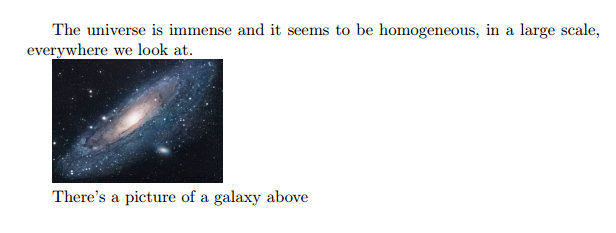
\includegraphics[width=8cm]{universe}
\end{center}

\subsection{User Characteristics}

*Provide here the characteristics of a typical user of the system (target
audience). List any technical background or expected prior experience.*  

\subsection{System's Functionality}

*Provide here an overview of the system and what the overall intention of the
system is.* 
      
\subsection{User Interfaces }

*Provide here a brief description of how the user will interact with the
system.*


\section{System Requirements}

\subsection{Functional Requirement}

*List here the functional requirements of the system. Functional requirements
are requirements that specify \textbf{what} the system should do and can be
thought of as 'the system must do \textit{requirement}'. Implementation details
for each requirement should be addressed in the system design document. An
example of a functional requirement would be 'the system utilizes Java
version...' This list can become quite extensive and for best practice each
requirement should be issued its own unique name, number, and be accompanied by
a description.*

\subsection{Non-Functional Requirement}

*List here the non-functional requirements of the system. Non-Functional
requirements are requirements that specify \textbf{how} the system should act
and can be thought of as 'the system shall be \textit{requirement}'. An example
of a non-functional requirement would be 'the system input should be able to
handle any file smaller than...'*

\end{document}

